\section{intro}
Considering that generative adversarial networks have straightforward latent space and allow various latent-based controls, similar understanding is necessary for diffusion models.


% Despite their success, the research community still lacks a clear understanding of what the latent variables or intermediate features of the models are embedded or how they are reflected in the resulting images. 
% \yh{
% We attribute it to the characteristic of the latent variable of DMs $\vx{}_t$ which is mere disruption of original images. As a result, it is not reasonable to expect any meaningful semantic structure in the latent space $\vx{}_t \in \mathcal{X}$.
% We attribute it to the characteristic of the latent variable of DMs $\vx{}_t$ which is disrupted image with gaussian noise. Therefore, we cannot expect any semantic structure in the latent space $\vx{}_t \in \mathcal{X}$.
% }

% \mingi{We attribute it to the characteristic iterative process of the DMs which involves a sequence of noisy images and subtle noises, i.e., the embeddings are not directly connected to the final images.}
% \mingi{Therefore, although we can regard the diffused noisy images, latent variables of DMs, as the latent space of DMs, the semantic adjustment method in the latent space has not been revealed.} 
% In contrast, arithmetic operations in the latent space of generative adversarial networks (GANs) lead to semantic changes in the resulting images \cite{goodfellow2020generative}. This property has been one of the key factors in developing GANs for real-world applications. We suppose that a better understanding of the latent space of DMs will boost similar development.

% \begin{figure}[!t]
%     \centering
%     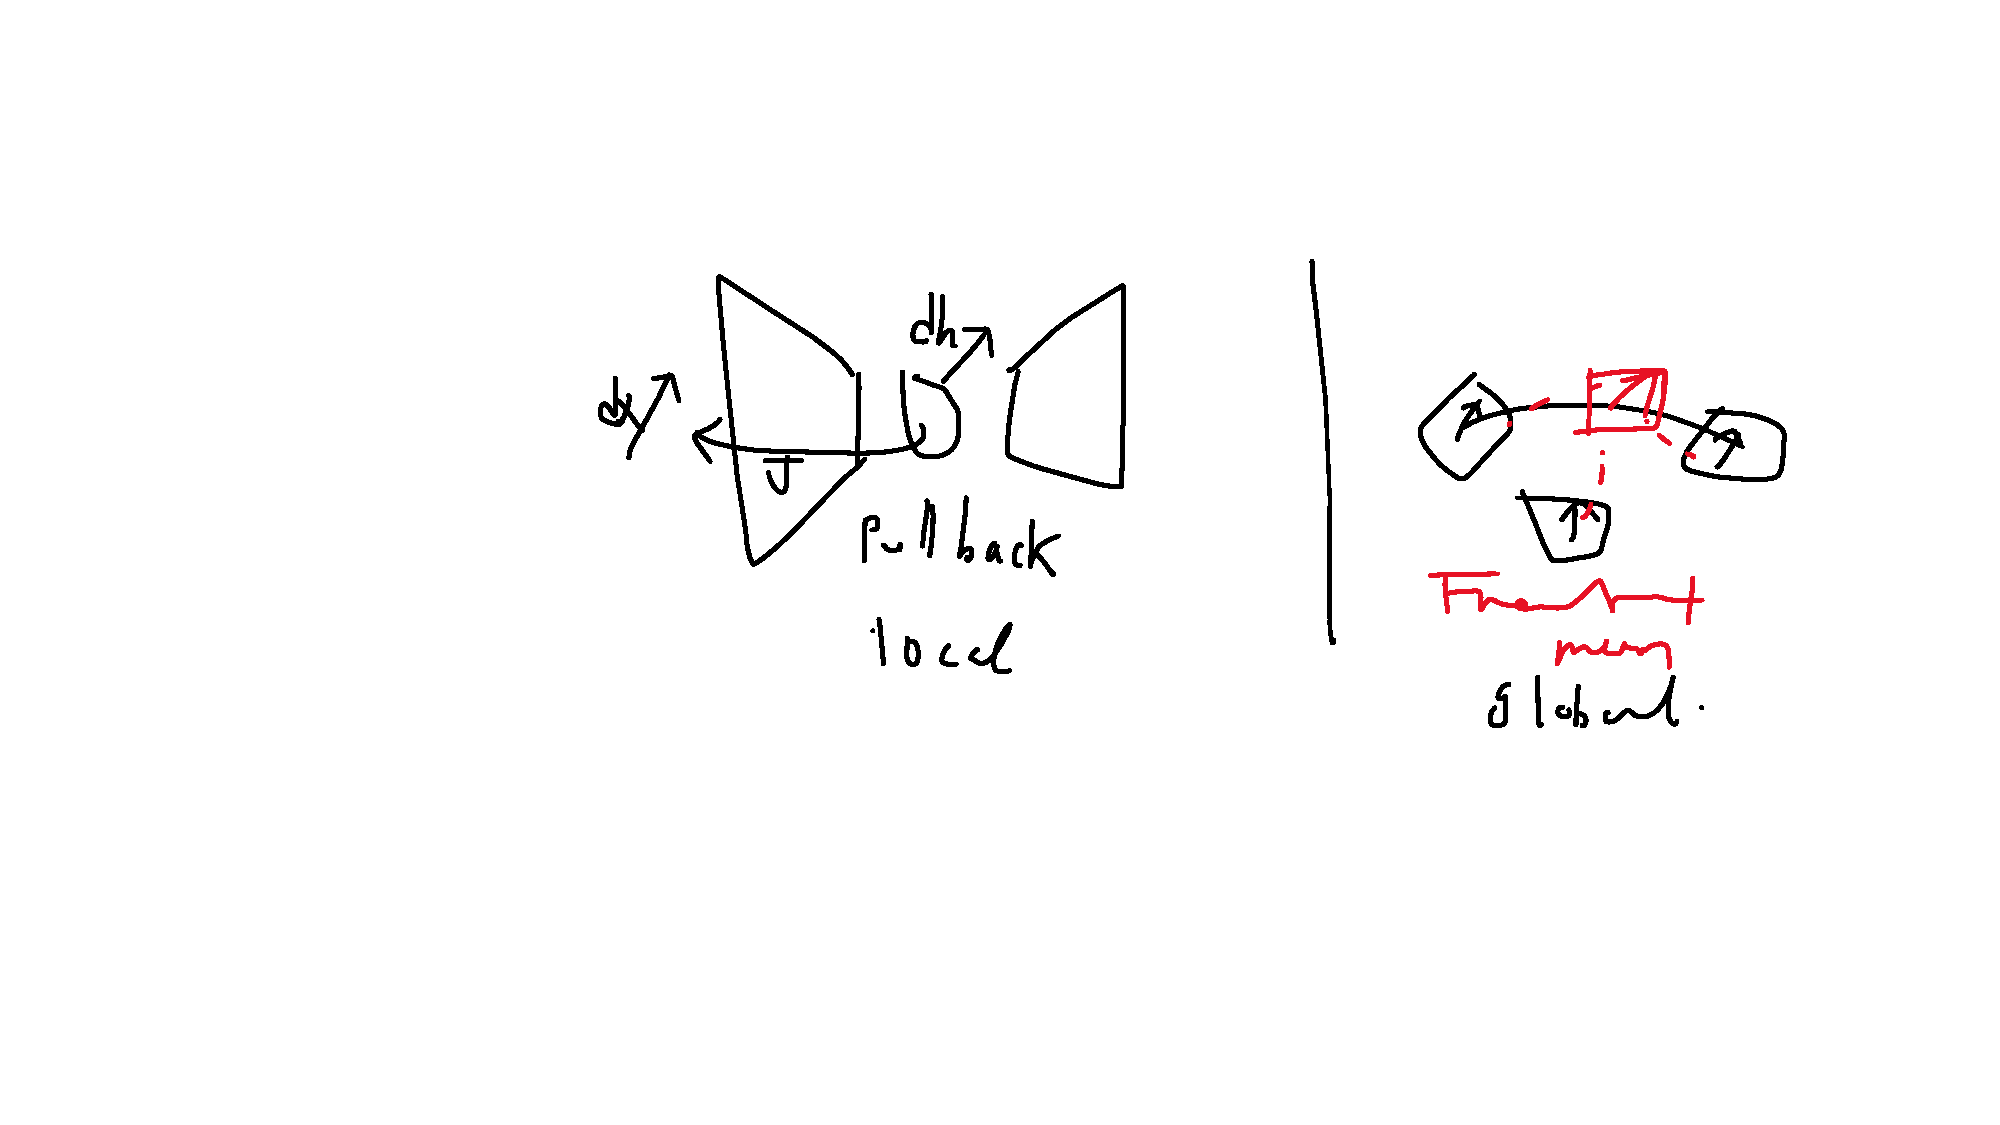
\includegraphics[width=0.9\linewidth]{./figure/method_explain.pdf}
%     \caption{\textbf{Conceptual illustration of our method.} 
%     전달 해야하는 정보 : 
%     1. pullback metric 을 통해 \exspace{}, \ehspace{} 에 local subspace 를 만든다
%     2. 서로 다른 sample 의 경우에는 parallel transport 로 옮겨다닌다.
%     3. x-space guidance 로 editing 한다. 
%     }
%     \vspace{-1em}
%     \label{fig:main_concept}
% \end{figure}


% \citet{kwon2022diffusion} adopt the intermediate feature space of the diffusion kernel as a semantic latent space, namely \ehspace{}, paired with a designated asymmetric sampling process. They revealed the local linearity of \ehspace{}.
% % , adding to our understanding of the latent space of DMs.
% However, they do not directly deal with the latent variables $\vx_t$ but rely only on a proxy, $\mathbf{h}$. 
% % Furthermore, they require external supervision such as Contrastive Language-Image Pretraining (CLIP) to find editable directions. \cite{radford2021learning}
% Since latent space \exspace{} is a sparse manifold, it is certainly not easy to do meaningful editing in it. However, \ehspace{} is clearly the codomain of \exspace{}, and the fact that we can find a meaningful semantic direction in \ehspace{} means that we can define semantic subspace in \exspace{} as well.


% \yh{Moreover, based on the observation that multiple samples exhibit comparable local semantic structures, we are able to create a global semantic basis using the \frechet{} mean.}
% \todo{check} 
% It follows the course of generative adversarial networks: extending per-sample editing directions \cite{ramesh2018spectral,patashnik2021styleclip,abdal2021styleflow,shen2021closed} to global editing directions \cite{harkonen2020ganspace,shen2021closed,yuksel2021latentclr}.

% \yh{
% Based on the observation that multiple samples exhibit comparable local semantic structures, we create a global semantic basis using the \frechet{} mean.
% It removes the cumbersome process of checking the semantic meaning of basis sample-by-sample and allows general controllability.
% It follows the course of generative adversarial networks: extending per-sample editing directions \cite{ramesh2018spectral,patashnik2021styleclip,abdal2021styleflow,shen2021closed} to global editing directions \cite{harkonen2020ganspace,shen2021closed,yuksel2021latentclr}.
% }

%\textcircled{\raisebox{-0.9pt}{1}} 
%\textcircled{\raisebox{-0.9pt}{2}} 
%\textcircled{\raisebox{-0.9pt}{3}} 
% We examined the evolution of the representation structure, i.e. local tangent basis, of DMs trained on various datasets. 
% We found that for DMs trained on simple, organized datasets such as CelebA-HQ and Flowers, there were regimes where the local tangent basis is similar between different diffusion timesteps. 
% We demonstrated that the model process similar signals through parallel transport. 
